\documentclass{article}
\usepackage[utf8]{inputenc}

\title{AAA Project}
%\author{Liron Mizrahi - 708810, Daniel da Silva - 738215, Jan Badenhorst - 707831}
\date{September 2016}

\author{
  Liron Mizrahi\\
  \texttt{708810}
  \and
  Daniel da Silva\\
  \texttt{738215}
  \and
  Jan Badenhorst\\
  \texttt{707831}
}


\usepackage{natbib}
\usepackage{graphicx}
\usepackage{algorithmic}
\usepackage{float}
\usepackage{hyperref}
\usepackage{booktabs}

\begin{document}

\maketitle

\section{Aims}
The problem proposed is to solve sudokus with a unique solution using the Backtracking Algorithm and to verify the theoretical analysis of the algorithm using empirical analysis.

\section{Summary of Theory}
A Backtracking algorithm is a type of brute force algorithm that incrementally builds candidates to the solution. If a candidate is found to be invalid, the algorithm 'backtracks' and deletes it. This only happens if the algorithm determines that the candidate cannot possibly lead to a solution.

\section{Experimental Methodology}
\subsection{Understanding the theoretical analysis}
The time complexity for this algorithm can be seen by working backwards from a single blank square. If there is only one blank square, then in the worst case there are $n$ possibilities that must be worked through. If there are two blank squares, then there are $n$ possibilities for the first square and $n$ possibilities for the second square corresponding to each of the possibilities for the first square. If there are three blank squares, then there are $n$ possibilities for the first blank. Each of those possibilities will lead to a puzzle with two blank squares that have $n^2$ possibilities.
The algorithm performs a depth first search through all the possible solutions. So carrying on in this way, the worst case complexity will end up being $O(n^m)$, where $n$ is the number of possibilities for each square and $m$ is the number of blank squares.

Using the number of iterations of the for loop in section 3.4 line 7 as the basic operation (alternatively and equivalently the number of times the IF statement is executed in section 3.4 line 8).

Some assertions to aid the analysis:
\begin{itemize}
	\item Line 13 will only occur if there was a number placed into an empty cell which is found to not fit into the solution in a following recursive call.
	\item In the event of line 13 occuring, the variable \emph{value} will be incremented by the for loop and inserted into the block.
	\item Once the new value is inserted, the algorithm iterates through all the other empty cells. 
\end{itemize}

The best case for this algorithm would be where all the missing blocks are low values. If that happens to be the case then there will be significantly less backtracking than if the missing values were higher. This can be clearly seen by using the simplifying assumption that the sudoku has a \emph{unique} solution. If only lower values are missing, and the solution is unique, the algorithm will clearly 'guess' the correct value sooner since it 'guesses' in ascending order from 1 to 9. To further clarify, if no 9's are missing, the algorithm will never have to guess 1, then 2, all the way up to 9. Hence fewer iterations of the for loop will be executed.

The worst case occurs if the missing numbers are generally higher values, since the algorithm may insert several, smaller numbers and have to backtrack repeatedly to get to a higher number. This means the for loop will have to be executed many times to increase the variable \emph{value} to the correct number. Note that for each of these 'guesses' the for loops will go through many more iterations for each following empty cell. Note here, the worst case does not occur if only higher numbers are missing. Due to the guesses being made using 1, 2, 3, ...,9, if no smaller numbers are missing, the algorithm will never try to insert the smaller numbers as it will always detect one in every cell's row, block or column.

For any case, the number of executions of our basic operation will be $O(n^m)$ where $n$ is the number of possible values for an empty cell and $m$ is the number of empty cells.

An exact complexity analysis of the best and worst cases is difficult, however it can be safely said that both cases have a complexity of $O(n^m)$, with best case having a lower value of $n$ than the worst case. This means both graphs are exponential however they do have different shapes with the best case being a slower increase with regards to the number of empty cells than the worst case.

\newpage

\subsection{Deciding on Appropriate Hardware and Programming Language}
The tests were run on a desktop PC with the following specifications:
\begin{itemize}
	\item \textbf{Processor:} Intel Core i3 6100 (3M cache, 3.70 GHz)
	\item \textbf{Ram:} 8GB DDR4
\end{itemize}

The programming language that has been chosen is C++, as it is much easier and more reliable to time the algorithm with the OpenMP library, rather than Java's timing implementations. Java would be easier to use for this sort of problem but the Garbage Collector may change results drastically and lead to incorrect results.

\subsection{Deciding on Appropriate Data Structures}
The data structure used is a three dimensional array. This is to store multiple sudokus from a text file. Prior to being passed to the backtracking algorithm, however, a sudoku is copied into a new two dimensional array. This is to reduce any additional memory access time required to reference the three dimensional array.

\newpage

\subsection{Implement the Algorithm}

    \begin{algorithmic}[1]
    %\Function{Increment}{$a$}
    
    \STATE Solve($int matrix[][]$)
        \STATE int $row$
        \STATE int $column$
\newline
        \IF {there are no empty squares} 
            \RETURN $true$
        \ENDIF
\newline
        \FOR{$value$ from $0$ \TO $9$}
            \IF{there are no numbers in same row, column and 3x3 square as $value$}
                \STATE $matrix[row][column]\gets value$
            
                \IF{Solve($matrix$)}
                    \RETURN $true$
                \ENDIF
                
                \STATE $matrix[row][column]\gets 0$
            \ENDIF
        \ENDFOR
\newline
        \RETURN $false$
    \STATE EndSolve
    %\EndFunction
\newline
    \end{algorithmic}

The algorithm above takes in a sudoku as a 2D matrix. The if statement on line 4 checks if there are any empty blocks in the matrix, if there are then $row$ and $column$ are assigned to the corresponding block. If there are no empty blocks then the sudoku is complete. 

The for loop on line 10 will iterate through the values $1$ to $9$ for the corresponding empty block. The if statement underneath checks if the current value can be placed in the block without breaking any of the rules of the sudoku. If it can be placed there then $matrix[row][column]$ is updated to the value.

The if statement on line 10 will recursively call the Solve function for $matrix$ with the newly inserted variable.
If any function call reaches line 13 then it means the current setup has failed and that the latest value must be backtracked. This line will reset the current block to 0. Line 16 is the line that invokes backtracking. When a $false$ value is returned then the previous block that was updated must be tried again for the other values it has not tried yet. If every function call returns true then the sudoku has been solved. If the first function call returns false then the sudoku has no solution.

\newpage

\subsection{Create the Data}
Data was generated using the website \url{https://kjell.haxx.se/sudoku/}. A field of 6 sudokus was generated for each number of completed cells from 17 up to 35. The sudokus were then converted into the required format. All the sudokus are claimed to have a unique solution.

It is extremely difficult to determine the layout of incomplete sudokus which should be used to create best or worst cases. For the best case, removing lower value numbers from a completed sudoku was considered however this could easily violate the assumption that we used in the theoretical analysis of the sudoku having a unique solution. For the worst case, violating the uniqueness is only half the problem; removing the higher numbers alone would not work as we would have to strategically remove smaller numbers as well. Determining which smaller numbers to remove and then deducing when a smaller number or larger number should be removed is no small task.

Faced with these issues the possibility of assessing several sudokus and then selecting sudokus with the metrics we desire was considered. It was found that the metrics commonly used involve invoking an algorithm to solve the sudoku and counting the number of iterations of a loop or the number of recursive calls. Higher iterations/recursive calls would indicate a harder sudoku (worst case) while lower would indicate an easier one (best case). Higher iterations/recursive calls would obviously also lead to higher run times. As such, it was found to be redundant to run a separate algorithm on the sudokus and being selective. When we consider further that it may take a huge number of tests to find a sudoku with the difficulty we need, we see that it would be easier to use the minimum and maximum runtimes of the sudokus for each number of empty cells as the best and worst cases respectively. This is proportional to the difficulty metrics commonly used. More data may be added to the text files for a better approximation in this regard.

A separate metric was designed to approximate the difficulty of the puzzles using the formula: \[\frac{number\_empty\_cells}{max\_number\_completed\_cells\_(block/row/column)}\]

This metric is useful in approximating the difficulty of the puzzle and was found to generally agree with the difficulty levels quoted by the website for each puzzle. However, our main analysis uses the number of empty cells vs time. This metric is just an attempt at evaluating what makes a sudoku difficult. Evaluation of the metric is done in sections 4.2 and 5.2.

\newpage

\section{Presentation of Results}
\subsection{Number of empty cells}
Firstly we examine the graphs of time vs number of empty cells.

\begin{figure}[H]
	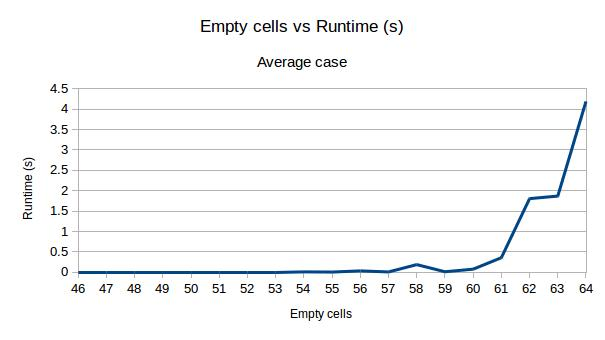
\includegraphics[width=0.9\linewidth, height=5cm]{graphs_outputs/EmptycellsVSTimeAverage.jpg}
	\caption{Average case}
\end{figure}

\begin{figure}[H]
	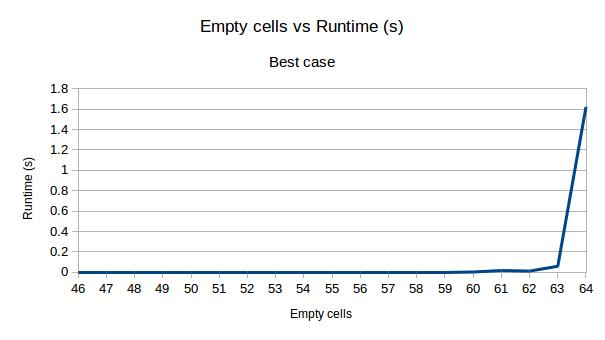
\includegraphics[width=0.9\linewidth, height=5cm]{graphs_outputs/EmptycellsVSTimeBest.jpg}
	\caption{Best case}
\end{figure}

\begin{figure}[H]
	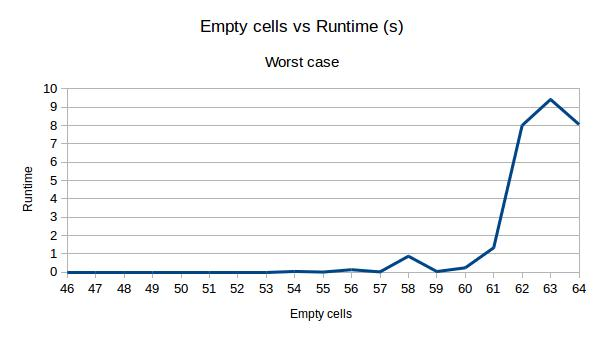
\includegraphics[width=0.9\linewidth, height=5cm]{graphs_outputs/EmptycellsVSTimeWorst.jpg}
	\caption{Worst case}
\end{figure}

\begin{figure}[H]
	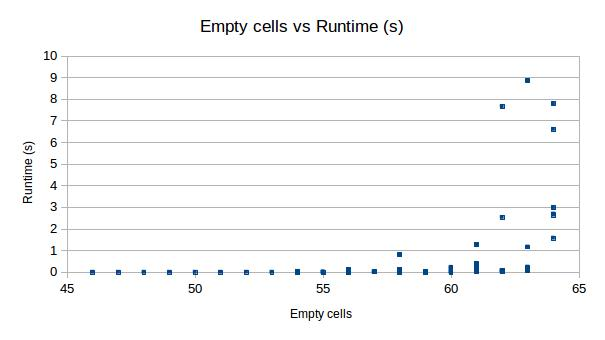
\includegraphics[width=0.9\linewidth, height=5cm]{graphs_outputs/EmptycellsVSTimeScatter.jpg}
	\caption{Scatter plot}
\end{figure}

\newpage

\subsection{Difficulty metric}
We now examine the test metric graphs to evaluate how good of an approximation it is for difficulty.

\begin{figure}[H]
	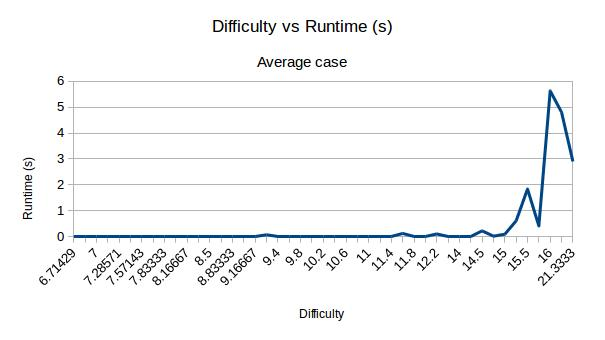
\includegraphics[width=0.9\linewidth, height=5cm]{graphs_outputs/DifficultyVSTimeAverage.jpg}
	\caption{Average case}
\end{figure}

\begin{figure}[H]
	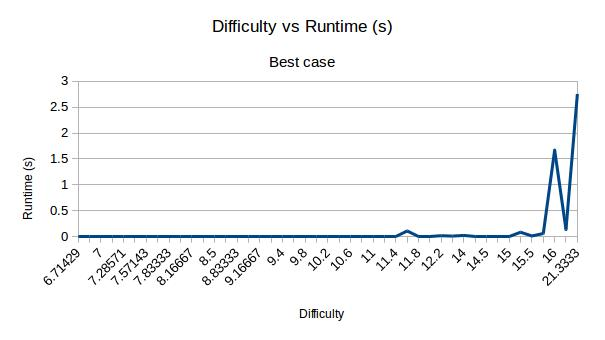
\includegraphics[width=0.9\linewidth, height=5cm]{graphs_outputs/DifficultyVSTimeBest.jpg}
	\caption{Best case}
\end{figure}

\begin{figure}[H]
	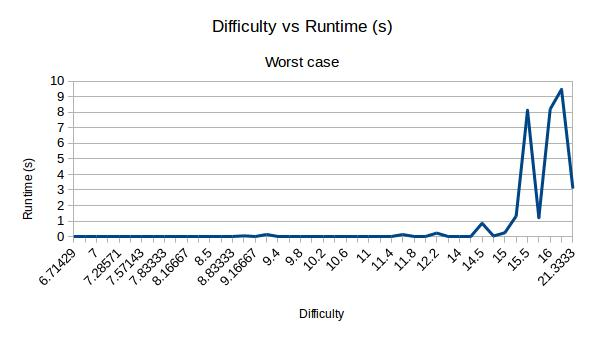
\includegraphics[width=0.9\linewidth, height=5cm]{graphs_outputs/DifficultyVSTimeWorst.jpg}
	\caption{Worst case}
\end{figure}

\begin{figure}[H]
	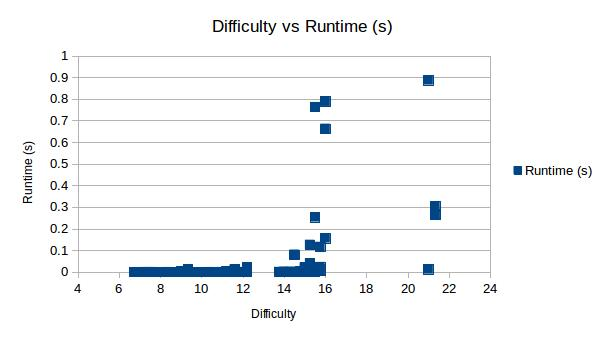
\includegraphics[width=0.9\linewidth, height=5cm]{graphs_outputs/DifficultyVSTimeScatter.jpg}
	\caption{Scatter plot}
\end{figure}

\newpage

\section{Interpretation of Results}
\subsection{Number of empty cells}
It is clear from figure 1 that there is a sharp increase in runtime from 61 empty cells to 64 empty cells. This growth is exponential. Note that sudokus with fewer than 17 numbers given will always have multiple solutions (See section 8 for more information). A somewhat small increase in runtime can be seen from 62 to 63 empty cells. We can ascertain that this is variation due to a few outliers as seen in figure 2. The number of sudokus taken into consideration for a given number of cells is only 6, so variations like these are to be expected. There is another variation in figure 1 at 58 empty cells. We can again ascertain that this is due to, in this case, a single outlier as seen in figure 2. There is a lot of variation in this problem as for some sudokus the algorithm may be 'lucky' and guess right multiple times without having to actually backtrack. As mentioned in the theoretical analysis, this occurs predominantly when the empty cells should contain lower numbers.

In all cases we see exponential growth. However, comparing the worst and best case graphs we see slower growth in the best case graph than in the worst case graph. The best case graph spikes at 64 empty cells, ie 17 numbers given which is something of a magic number in terms of sudokus in that sudokus are known to be much more difficult to solve when only 17 numbers are given.

It is important to note the small runtimes for 46 to 56 empty cells, which provide small changes that cannot be viewed in figure 1 due to the scaling. Refer to figure 9 below for the graph of that region.

\begin{figure}[H]
	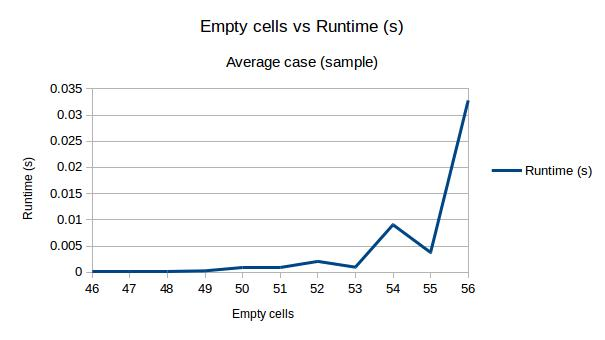
\includegraphics[width=0.9\linewidth, height=5cm]{graphs_outputs/EmptycellsVSTimeAverage(Sample).jpg}
	\caption{Aggregated data Empty cells vs time for 46-57}
\end{figure}

Here we see an exponential relation as well, which again, appears as a relatively straight line on the graph in figure 1. This really outlines the magnitude with which the runtime increased in figure 1.

\newpage

\subsection{Difficulty metric}
The difficulty metric mostly mirrors the number of empty cells graphs, however there are much larger variations in the graphs and the mirroring likely only occurs because the number of empty cells actively part-takes in the formula. The metric was designed to take into account difficulty a human would have in solving a sudoku as opposed to what the algorithm might struggle with. It does not seem to provide a better approximation than the number of empty cells. Notice the large variation right at the end of the graph (at around 21 difficulty units), this is clearly a sudoku being rated as quite difficult when it should not be considered as such. This is why the metric is not considered in the empirical analysis although the graphs are provided for interest's sake.

\section{Relate results to Theory}
As we can see in all the graphs, an exponential growth rate is present. This agrees with the theoretical analysis. Also agreeing with the theoretical analysis, we see that the best case has a smaller constant ($n$ in the theoretical analysis) than the worst case. This can only be due to fewer backtracks in the best case since the number of empty cells is held constant.

\section{Conclusion}
\subsection{Algorithm}
As shown by the graphs and the theoretical analysis, the time complexity of the backtracking algorithm is $O(n^m)$, which is exponential. This is not a very efficient algorithm, but when working with 9x9 grids the complexity is not very obvious. The backtracking approach to sudoku puzzles should perform a lot more efficiently than primitive brute force as it eliminates a lot of possible attempts.

\subsection{Experimental Methodology Evaluation}
It is unfortunate that the test data could not be designed to create best and worst cases as per traditional Empirical Analysis however, using the minimum and maximum times results in a good confirmation of the analysis done despite this setback. More sudokus could have been used to provide better graphs in best, worst and average cases.

\newpage
\section{Unique Solutions and 17 - Discussion}
As stated in section 5.1, a sudoku with fewer than 17 numbers has been proven to \emph{always} have multiple solutions. This is noteworthy because of how and when it was proved. It was proved as recently as the 1$^{st}$ of January, 2012 and was done so using an exhaustive technique. The algorithm designed was run on a supercomputer at the Irish Centre for High-End Computing (ICHEC) and took about 12 months to complete. The algorithm involved taking completed sudokus and trying to extract an incomplete sudoku with 16 numbers given that leads to a unique solution. None was found, proving that unique solution sudokus with 16 clues given are not possible. The paper can be found here: \url{https://arxiv.org/pdf/1201.0749v2.pdf}.

\section{Acknowledgments}
Thank you to Kjell Ericson for the test data which is created on demand at https://kjell.haxx.se/sudoku/.

\section{References}
\url{https://en.wikipedia.org/wiki/Sudoku_solving_algorithms} \\
\url{https://codemyroad.wordpress.com/2014/05/01/solving-sudoku-by-backtracking/}
\url{https://arxiv.org/pdf/1201.0749v2.pdf}\\

\begin{table}[H]
	\centering
	\begin{tabular}{|c|c|c|}
		\hline
		Liron Mizrahi & Daniel da Silva & Jan Badenhorst  \\ \hline
		33\%  & 33\%   & 33\% \\ \hline
	\end{tabular}
	\caption{Statement of Effort}
	\label{my-label}
\end{table}

\end{document}
